\documentclass[tikz,border=10pt]{standalone}

\begin{document}
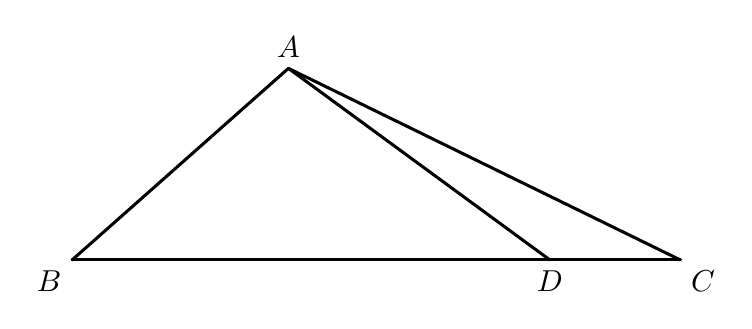
\begin{tikzpicture}[line width=1.1pt, line join=round, line cap=round]
\coordinate (A) at (-1.116,1.226);
\coordinate (B) at (-3.863,-1.207);
\coordinate (C) at (3.860,-1.207);
\coordinate (D) at (2.204,-1.207);

  
  \draw[solid] (A) -- (B);
  \draw[solid] (A) -- (C);
  \draw[solid] (A) -- (D);
  
  \draw[solid] (B) -- (D) -- (C);

  
  \node[above, font=\fontsize{10.5}{12.6}\selectfont] at (A) {$A$};
  \node[below left, font=\fontsize{10.5}{12.6}\selectfont] at (B) {$B$};
  \node[below, font=\fontsize{10.5}{12.6}\selectfont] at (D) {$D$};
  \node[below right, font=\fontsize{10.5}{12.6}\selectfont] at (C) {$C$};
\end{tikzpicture}
\end{document}